\documentclass[a4paper]{ctexart}
\usepackage[top = 2cm, bottom = 2cm, left = 2cm, right = 2cm]{geometry}
\usepackage{amsmath, amssymb, amsthm, tikz, pgfplots, float}

\tikzset{elegant/.style={smooth,thick,solid,black}}
\tikzset{eaxis/.style={smooth,thick,solid,black}}

\title{Homework for Chapter 3}
\author{数学与应用数学(强基计划)\qquad 王笑同\qquad 3210105450}
\date{\today}

\begin{document}

\maketitle
\textbf{Problem 1.}

\begin{proof}[Solution]
	The polynomial $p(x)$ must meet the conditions:
	$$
		p(0)=0, \ p(1)=1, \ p'(1)=-3, \ p''(1)=6.
	$$
	Applying Hermite interpolation yields:
	$$
		p(x)=7x^3-18x^2+12x.
	$$
	The spline $s(x)$ does not qualify as a natural cubic spline because $s''(0)=-36\neq 0$.
\end{proof}

\textbf{Problem 2.}

\begin{proof}[Solution]
	(a) Let $p_i=s|_{[x_i,x_{i+1}]}\in\mathbb{P}_2$, introducing $3(n-1)$ unknowns in $p_1,...,p_{n-1}$. The following equations
	$$
		p_i(x_i)=f_i, \ p_i(x_{i+1})=f_{i+1}, \ i=1,...,n-1
	$$
	generate $2(n-1)$ conditions. Additionally,
	$$
		p'_i(x_{i+1})=p'_{i+1}(x_{i+1}), \ i=1,...,n-2
	$$
	provide $n-2$ more conditions. Thus, there are $3(n-1)$ unknowns and $3(n-1)-1$ equations.

	An extra condition is therefore required.

	(b) Assuming $p_i(x)=a_ix^2+b_ix+c_i$, we derive from the conditions:
	$$
		\begin{cases}
			x_i^2a_i+x_ib_i+c_i=f_i             \\
			x_{i+1}^2a_i+x_{i+1}b_i+c_i=f_{i+1} \\
			2x_ia_i+b_i=m_i
		\end{cases}
	$$
	Solving for $a_i,b_i,c_i$ gives:
	\begin{align*}
		a_i & =\frac{f_{i+1}-f_i}{(x_{i+1}-x_i)^2}-\frac{m_i}{x_{i+1}-x_i},                        \\
		b_i & =\frac{m_i(x_{i+1}+x_i)}{x_{i+1}-x_i}-\frac{2x_i(f_{i+1}-f_i)}{(x_{i+1}-x_i)^2},     \\
		c_i & =f_i+\frac{x_i^2(f_{i+1}-f_i)}{(x_{i+1}-x_i)^2} - \frac{m_ix_ix_{i+1}}{x_{i+1}-x_i}.
	\end{align*}
	Thus $p_i$ is uniquely defined.

	(c) Determine $p_1$ using $f_1,f_2,m_1$. Set $m_2=p'_1(x_2)$.

	Find $p_2$ using $f_2,f_3,m_2$. Set $m_3=p'_2(x_3)$.

	$\vdots$

	Finally, find $p_{n-1}$ using $f_{n-1},f_n,m_{n-1}$.

\end{proof}

\textbf{Problem 3.}

\begin{proof}[Solution]
	Consider $s_2(x)=\alpha x^3+\beta x^2+\gamma x+\theta$. The following must hold:
	$$
		s_2(0)=s_1(0)=1+c, \ s'_2(0)=s'_1(0)=3c, \ s''_2(0)=s''_1(0)=6c, \ s_2(1)=s(1)=-1, \ s''_2(1)=0.
	$$
	These yield:
	$$
		\begin{cases}
			\theta = 1+c,                    \\
			\gamma = 3c,                     \\
			2\beta = 6c,                     \\
			\alpha+\beta+\gamma+\theta = -1, \\
			6\alpha+2\beta=0
		\end{cases}.
	$$
	Solving this system gives $c=-\frac{1}{3}$.
\end{proof}

\textbf{Problem 4.}

\begin{proof}[Solution]
	(a) The natural cubic spline interpolating $f$ at knots $-1,0,1$ is:
	$$
		s(x)=\begin{cases}
			-\frac{1}{2}x^3-\frac{3}{2}x^2+1 & \text{for } x\in[-1,0], \\
			\frac{1}{2}x^3-\frac{3}{2}x^2+1  & \text{for } x\in[0,1].
		\end{cases}
	$$

	(b) The bending energy of $s$ is calculated as:
	$$
		\int_{-1}^1 [s''(x)]^2 \, dx = \int_{-1}^0 (-3x-3)^2 \, dx + \int_{0}^1 (3x-3)^2 \, dx=6.
	$$

	The quadratic polynomial interpolating $f$ at $-1,0,1$ is:
	$$
		p(x)=-x^2+1.
	$$
	Its bending energy is:
	$$
		\int_{-1}^1 [p''(x)]^2 \, dx = \int_{-1}^1 4 \, dx = 8 > 6.
	$$

	The bending energy of $f$ is:
	$$
		\int_{-1}^1 [f''(x)]^2 \, dx = \int_{-1}^1 \left[-\frac{\pi^2}{4}\cos\left(\frac{\pi}{2}x\right)\right]^2 \approx \frac{\pi^4}{16} \approx 6.0881 > 6.
	$$
\end{proof}


\textbf{Problem 5.}

\begin{proof}[Solution]
	\begin{itemize}
		\item See that
		      $$
			      B_i^1(x)=\left\{ \begin{array}{ll}
				      \frac{x-t_{i-1}}{t_i-t_{i-1}} & x\in(t_{i-1},t_i], \\
				      \frac{t_{i+1}-x}{t_{i+1}-t_i} & x\in(t_i,t_{i+1}], \\
				      0                             & \text{otherwise}.
			      \end{array} \right. \qquad
			      B_{i+1}^1(x)=\left\{ \begin{array}{ll}
				      \frac{x-t_{i}}{t_{i+1}-t_{i}}     & x\in(t_{i},t_{i+1}],   \\
				      \frac{t_{i+2}-x}{t_{i+2}-t_{i+1}} & x\in(t_{i+1},t_{i+2}], \\
				      0                                 & \text{otherwise}.
			      \end{array} \right.
		      $$
		      And by the recursive definition we have
		      $$
			      B_i^2(x)=\frac{x-t_{i-1}}{t_{i+1}-t_{i-1}}B_i^1(x)+\frac{t_{i+2}-x}{t_{i+2}-t_{i}}B_{i+1}^1(x)
		      $$
		      For $x\in(t_{i-1},t_i]$,
		      $$
			      B_i^2(x)=\frac{x-t_{i-1}}{t_{i+1}-t_{i-1}}\cdot \frac{x-t_{i-1}}{t_i-t_{i-1}}+\frac{t_{i+2}-x}{t_{i+2}-t_{i}}\cdot 0 = \frac{(x-t_{i-1})^2}{(t_{i+1}-t_{i-1})(t_i-t_{i-1})}.
		      $$
		      For $x\in(t_{i},t_{i+1}]$,
		      $$
			      B_i^2(x)=\frac{(x-t_{i-1})(t_{i+1}-x)}{(t_{i+1}-t_{i-1})(t_{i+1}-t_i)}+\frac{(t_{i+2}-x)(x-t_i)}{(t_{i+2}-t_{i})(t_{i+1}-t_{i})}.
		      $$
		      For $x\in(t_{i+1},t_{i+2}]$,
		      $$
			      B_i^2(x)=\frac{x-t_{i-1}}{t_{i+1}-t_{i-1}}\cdot 0+\frac{t_{i+2}-x}{t_{i+2}-t_{i}}\cdot \frac{t_{i+2}-x}{t_{i+2}-t_{i+1}} = \frac{(t_{i+2}-x)^2}{(t_{i+2}-t_{i})(t_{i+2}-t_{i+1})}.
		      $$
		      Hence we derived
		      \begin{equation}
			      B_i^2(x)=\left\{ \begin{array}{ll}
				      \frac{(x-t_{i-1})^2}{(t_{i+1}-t_{i-1})(t_i-t_{i-1})}                                                                    & x\in(t_{i-1},t_i],     \\
				      \frac{(x-t_{i-1})(t_{i+1}-x)}{(t_{i+1}-t_{i-1})(t_{i+1}-t_i)}+\frac{(t_{i+2}-x)(x-t_i)}{(t_{i+2}-t_{i})(t_{i+1}-t_{i})} & x\in(t_i,t_{i+1}],     \\
				      \frac{(t_{i+2}-x)^2}{(t_{i+2}-t_{i})(t_{i+2}-t_{i+1})}                                                                  & x\in(t_{i+1},t_{i+2}], \\
				      0                                                                                                                       & \text{otherwise}.
			      \end{array} \right.
		      \end{equation}

		\item We have
		      \begin{equation}
			      \frac{\text{d}}{\text{d}x}B_i^2(x)=\left\{ \begin{array}{ll}
				      p_1(x)=\frac{2(x-t_{i-1})}{(t_{i+1}-t_{i-1})(t_i-t_{i-1})}                                                             & x\in(t_{i-1},t_i],     \\
				      p_2(x)=\frac{t_{i+1}+t_{i-1}-2x}{(t_{i+1}-t_{i-1})(t_{i+1}-t_i)}+\frac{t_{i+2}+t_i-2x}{(t_{i+2}-t_{i})(t_{i+1}-t_{i})} & x\in(t_i,t_{i+1}],     \\
				      p_3(x)=\frac{2(x-t_{i+2})}{(t_{i+2}-t_{i})(t_{i+2}-t_{i+1})}                                                           & x\in(t_{i+1},t_{i+2}], \\
				      0                                                                                                                      & \text{otherwise}.
			      \end{array} \right.
		      \end{equation}
		      We have
		      \begin{align*}
			      p_1(t_i) & =\frac{2(t_i-t_{i-1})}{(t_{i+1}-t_{i-1})(t_i-t_{i-1})}=\frac{2}{t_{i+1}-t_{i-1}}                                     \\
			      p_2(t_i) & =\frac{t_{i+1}+t_{i-1}-2t_i}{(t_{i+1}-t_{i-1})(t_{i+1}-t_i)}+\frac{t_{i+2}+t_i-2t_i}{(t_{i+2}-t_{i})(t_{i+1}-t_{i})} \\
			               & =\frac{t_{i-1}-t_i}{(t_{i+1}-t_{i-1})(t_{i+1}-t_i)}+\frac{1}{t_{i+1}-t_{i-1}}+\frac{1}{t_{i+1}-t_{i}}                \\
			               & =\frac{t_{i-1}-t_i+t_{i+1}-t_{i-1}}{(t_{i+1}-t_{i-1})(t_{i+1}-t_i)}+\frac{1}{t_{i+1}-t_{i-1}}                        \\
			               & =\frac{2}{t_{i+1}-t_{i-1}} = p_1(t_i)
		      \end{align*}
		      Hence $\frac{\text{d}}{\text{d}x}B_i^2(x)$ is continuous at $t_i$. Similarly,
		      \begin{align*}
			      p_3(t_{i+1}) & =\frac{2(t_{i+1}-t_{i+2})}{(t_{i+2}-t_{i})(t_{i+2}-t_{i+1})}=-\frac{2}{t_{i+2}-t_{i}}                                                                              \\
			      p_2(t_{i+1}) & =\frac{t_{i+1}+t_{i-1}-2t_{i+1}}{(t_{i+1}-t_{i-1})(t_{i+1}-t_i)}+\frac{t_{i+2}+t_i-2t_{i+1}}{(t_{i+2}-t_{i})(t_{i+1}-t_{i})}=-\frac{2}{t_{i+2}-t_{i}}=p_3(t_{i+1})
		      \end{align*}
		      Hence $\frac{\text{d}}{\text{d}x}B_i^2(x)$ is continuous at $t_{i+1}$.

		\item We konw $\frac{\text{d}}{\text{d}x}B_i^2(x)$ is continuous, and is a linear function at each interval $(t_{i-1},t_i],(t_{i},t_{i+1}]$ and $(t_{i+1},t_{i+2}]$. And we have that
		      $$
			      \frac{\text{d}}{\text{d}x}B_i^2(t_{i-1})=0,\qquad \frac{\text{d}}{\text{d}x}B_i^2(t_i)=\frac{2}{t_{i+1}-t_{i-1}}>0.
		      $$
		      So by the property of linear function,
		      $$
			      \frac{\text{d}}{\text{d}x}B_i^2(x)>0, \quad x\in(t_{i-1},t_i]
		      $$
		      Morever,
		      $$
			      \frac{\text{d}}{\text{d}x}B_i^2(t_{i+1})=-\frac{2}{t_{i+2}-t_i}<0
		      $$
		      Hence by the property of linear function, there is unique $x^*\in(t_{i},t_{i+1})$ such that $\frac{\text{d}}{\text{d}x}B_i^2(x^*)=0$. It follows the below eqution.
		      $$
			      \frac{t_{i+1}+t_{i-1}-2x^*}{t_{i+1}-t_{i-1}}+\frac{t_{i+2}+t_i-2x^*}{t_{i+2}-t_i}=0
		      $$
		      Solve it and we got
		      $$
			      x^*=\frac{t_{i+2}t_{i+1}-t_it_{i-1}}{(t_{i+2}+t_{i+1})-(t_i+t_{i-1})}.
		      $$

		\item By (c) we know that:
		      \begin{align*}
			       & \frac{\text{d}}{\text{d}x}B_i^2(x)>0, \quad x\in(t_{i-1},x^*) \\
			       & \frac{\text{d}}{\text{d}x}B_i^2(x)<0, \quad x\in(x^*,t_{i+2})
		      \end{align*}
		      Also $B_i^2(t_{i-1})=B_i^2(t_{i+2})=0$. And $B(x^*)<1$ could be verified by a trivial computation. Hence $B_i^2(x)\in[0,1)$.

		\item Clearly the image of $B_i^2(x)$ with different $i$ could be obtained by translation. So we just draw with $i=0$.
		      \begin{center}
			      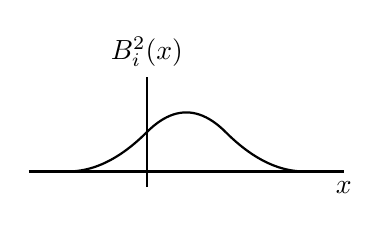
\begin{tikzpicture}
				      % draw the axis
				      \draw[eaxis] (-1.5,0) -- (2.5,0) node[below] {$x$};
				      \draw[eaxis] (0,-0.2) -- (0,1.2) node[above] {$B_i^2(x)$};
				      % draw the function (piecewise)
				      \draw[elegant,domain=-1.5:-1] plot(\x,0);
				      \draw[elegant,domain=-1:0] plot(\x,{(\x+1)^2/2});
				      \draw[elegant,domain=0:1] plot(\x,{(\x+1)*(1-\x)/2+(2-\x)*\x/2});
				      \draw[elegant,domain=1:2] plot(\x,{(2-\x)^2/2});
				      \draw[elegant,domain=2:2.5] plot(\x,0);
			      \end{tikzpicture}
		      \end{center}
	\end{itemize}
\end{proof}

\textbf{Problem 6.}

\begin{proof}[Solution]
	For $x\in(t_{i-1},t_i]$, by Lagrange's formula we have:
	\begin{align*}
		[t_{i-1},t_i,t_{i+1},t_{i+2}](t-x)_+^2= & \frac{(t_i-x)^2}{(t_i-t_{i-1})(t_{i}-t_{i+1})(t_i-t_{i+2})}+\frac{(t_{i+1}-x)^2}{(t_{i+1}-t_{i-1})(t_{i+1}-t_{i})(t_{i+1}-t_{i+2})} \\
		                                        & +\frac{(t_{i+2}-x)^2}{(t_{i+2}-t_{i-1})(t_{i+2}-t_{i})(t_{i+2}-t_{i+1})}                                                            \\
		=                                       & \frac{(x-t_{i-1})^2}{(t_{i+2}-t_{i-1})(t_{i+1}-t_{i-1})(t_i-t_{i-1})}=\frac{B_i^2(x)}{t_{i+2}-t_{i-1}}
	\end{align*}
	For $x\in(t_{i},t_{i+1}]$, by Lagrange's formula we have:
	\begin{align*}
		[t_{i-1},t_i,t_{i+1},t_{i+2}](t-x)_+^2= & \frac{(t_{i+1}-x)^2}{(t_{i+1}-t_{i-1})(t_{i+1}-t_{i})(t_{i+1}-t_{i+2})}+\frac{(t_{i+2}-x)^2}{(t_{i+2}-t_{i-1})(t_{i+2}-t_{i})(t_{i+2}-t_{i+1})} \\
		=                                       & \frac{B_i^2(x)}{t_{i+2}-t_{i-1}}
	\end{align*}
	For $x\in(t_{i+1},t_{i+2}]$, by Lagrange's formula we have:
	\begin{align*}
		[t_{i-1},t_i,t_{i+1},t_{i+2}](t-x)_+^2= & \frac{(t_{i+2}-x)^2}{(t_{i+2}-t_{i-1})(t_{i+2}-t_{i})(t_{i+2}-t_{i+1})} \\
		=                                       & \frac{B_i^2(x)}{t_{i+2}-t_{i-1}}
	\end{align*}
	Hence we verified
	$$
		(t_{i+2}-t_{i-1})[t_{i-1},t_i,t_{i+1},t_{i+2}](t-x)_+^2=B_i^2(x)
	$$
	in the support of $B_i^2(x)$. And clearly, the equation is also right when $B_i^2(x)$ vanishes.
\end{proof}

\textbf{Problem 7.}

\begin{proof}[Solution]
	By the Theorem on derivates of B-splines, we have
	$$
		\frac{\text{d}}{\text{d}x}B_i^{n+1}(x)=\frac{(n+1)B_i^{n}(x)}{t_{i+n}-t_{i-1}}-\frac{(n+1)B_{i+1}^{n}(x)}{t_{i+n+1}-t_i} ,\qquad n=1,2,...
	$$
	Integral to both side, we have:
	$$
		\int_{t_{i-1}}^{t_{i+n+1}}\frac{\text{d}}{\text{d}x}B_i^{n+1}(x) \text{d}x=\int_{t_{i-1}}^{t_{i+n+1}}\frac{(n+1)B_i^{n}(x)}{t_{i+n}-t_{i-1}}-\frac{(n+1)B_{i+1}^{n}(x)}{t_{i+n+1}-t_i}\text{d} x,\qquad n=1,2,...
	$$
	For the left side, we have:
	$$
		\text{LHS}=B_i^{n+1}(t_{i+n+1})-B_i^{n+1}(t_{i-1})=0-0=0.
	$$
	For the right side, we have:
	$$
		\text{RHS}=(n+1)\left(\int_{t_{i-1}}^{t_{i+n}}\frac{B_i^{n}(x)}{t_{i+n}-t_{i-1}} \text{d}x-\int_{t_{i}}^{t_{i+n+1}}\frac{B_{i+1}^{n}(x)}{t_{i+n+1}-t_{i}} \text{d}x\right)
	$$
	Then we got
	$$
		\int_{t_{i-1}}^{t_{i+n}}\frac{B_i^{n}(x)}{t_{i+n}-t_{i-1}} \text{d}x=\int_{t_{i}}^{t_{i+n+1}}\frac{B_{i+1}^{n}(x)}{t_{i+n+1}-t_{i}} \text{d}x
	$$
	Hence the scaled integral of $B_i^n(x)$ over its support is independent of $i$.
\end{proof}

\textbf{Problem 8.}

\begin{proof}[Solution]
	\begin{enumerate}[(a)]
		\item By the definition,
		      $$
			      \tau_2(x_i,x_{i+1},x_{i+2})=x_i^2+x_{i+1}^2+x_{i+2}^2+x_ix_{i+1}+x_ix_{i+2}+x_{i+1}x_{i+2}.
		      $$
		      Make a table of divided difference as following.
		      \begin{table}[H]
			      \centering
			      \begin{tabular}{l|lll}
				      $x_i$     & $x_i^4$     &                                          &                                                                                                 \\
				      $x_{i+1}$ & $x_{i+1}^4$ & $(x_{i+1}^2+x_{i}^2)(x_{i+1}+x_{i})$     &                                                                                                 \\
				      $x_{i+2}$ & $x_{i+2}^4$ & $(x_{i+2}^2+x_{i+1}^2)(x_{i+2}+x_{i+1})$ & $\frac{(x_{i+2}^2+x_{i+1}^2)(x_{i+2}+x_{i+1})-(x_{i+1}^2+x_{i}^2)(x_{i+1}+x_{i})}{x_{i+2}-x_i}$
			      \end{tabular}
		      \end{table}
		      Then the result follows from
		      \begin{align*}
			        & \frac{(x_{i+2}^2+x_{i+1}^2)(x_{i+2}+x_{i+1})-(x_{i+1}^2+x_{i}^2)(x_{i+1}+x_{i})}{x_{i+2}-x_i} \\
			      = & \frac{(x_{i+2}^3-x_i^3)+x_{i+1}(x_{i+2}^2-x_i^2)+x_{i+1}^2(x_{i+2}-x_i)}{x_{i+2}-x_i}         \\
			      = & (x_{i+2}^2+x_{i+2}x_i+x_i^2)+x_{i+1}(x_{i+2}+x_i)+x_{i+1}^2                                   \\
			      = & \tau_2(x_i,x_{i+1}+x_{i+2}).
		      \end{align*}

		\item By the lemma on recursive relations of complete symmetric polynomials, we have
		      \begin{align*}
			        & (x_{i+n+1}-x_i)\tau_{m-n-1}(x_i,...,x_{i+n+1})                                                                                      \\
			      = & \tau_{m-n}(x_i,...,x_{i+n+1})-\tau_{m-n}(x_i,...,x_{i+n})-x_i\tau_{m-n-1}(x_i,...,x_{i+n+1})                                        \\
			      = & \tau_{m-n}(x_{i+1},...,x_{i+n+1})+x_i\tau_{m-n-1}(x_i,...,x_{i+n+1})-\tau_{m-n}(x_i,...,x_{i+n})-x_i\tau_{m-n-1}(x_i,...,x_{i+n+1}) \\
			      = & \tau_{m-n}(x_{i+1},...,x_{i+n+1})-\tau_{m-n}(x_i,...,x_{i+n}).
		      \end{align*}
		      Now we prove the theorem by induction. For $n=0$, clearly
		      $$
			      \tau_m(x_i)=[x_i]x^m=x_i^m.
		      $$
		      Now we suppose the theorem is true for some $0\leq n<m$. Then for $n+1$, we have
		      \begin{align*}
			      \tau_{m-n-1}(x_i,...,x_{i+n+1}) & =\frac{\tau_{m-n}(x_{i+1},...,x_{i+n+1})-\tau_{m-n}(x_i,...,x_{i+n})}{x_{i+n+1}-x_{i}} \\
			                                      & =\frac{[x_{i+1},...,x_{i+n+1}]x^m-[x_i,...,x_{i+n}]}{x_{i+n+1}-x_{i}}                  \\
			                                      & =[x_i,...,x_{i+n+1}]x^m
		      \end{align*}
		      Then the theorem is proved by induction.
	\end{enumerate}
\end{proof}
\end{document}